\documentclass{article}

\usepackage{pgf}
\usepackage{tikz}
\usetikzlibrary{arrows, automata}
\begin{document}
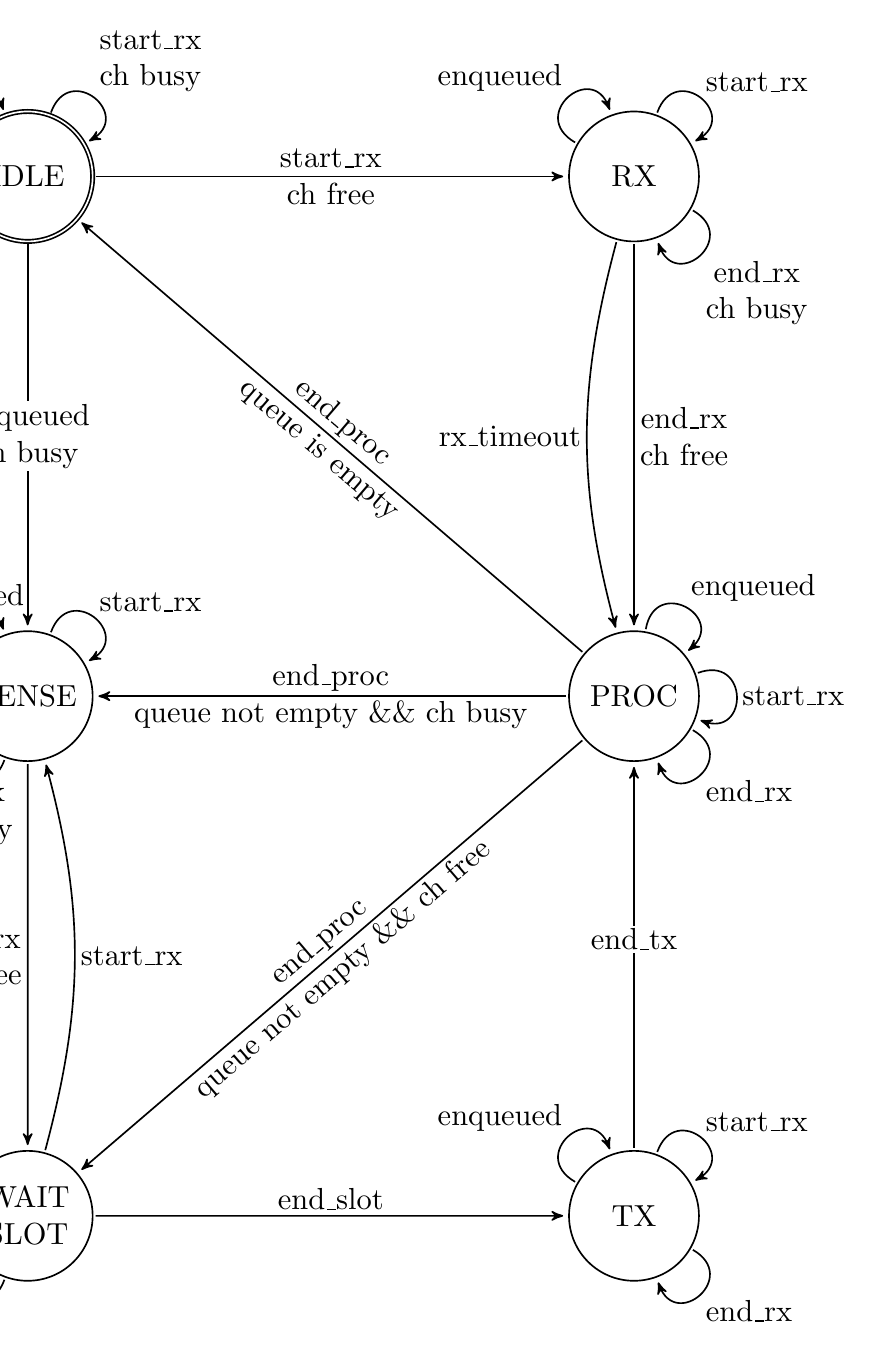
\begin{tikzpicture}[->, >=stealth', shorten >=1pt, auto, node
    distance=6cm, trim left, semithick, outer sep=1pt, inner sep=1pt,
    every node/.style={scale=1.1}, align=center]

  \tikzstyle{every state}=[minimum size=1.5cm]

  \node[state,double] (IDLE) {IDLE};
  \node[state, node distance=7cm] (RX) [right of=IDLE] {RX};
  \node[state]         (SENSE) [below of=IDLE] {SENSE};
  \node[state]         (PROC) [below of=RX] {PROC};
  \node[state]         (SLOT) [below of=SENSE] {WAIT\\SLOT};
  \node[state]         (TX) [below of=PROC] {TX};

  \path[->]
  (IDLE) edge [anchor=center] node {start\_rx\\ch free} (RX)
  edge [anchor=center] node [fill=white] {enqueued\\ch busy} (SENSE)
  edge [anchor=center, out=-120, in=120, looseness=0.9] node
  [fill=white] {enqueued\\ch free} (SLOT)
  edge [out=150,in=110,loop, looseness=3] node {end\_rx} (IDLE)
  edge [out=70,in=30,loop, looseness=3] node {start\_rx\\ch busy} (IDLE)

  (RX) edge node {end\_rx\\ch free} (PROC)
  edge [out=150,in=110,loop, looseness=3] node {enqueued} (RX)
  edge [out=70, in=30, loop, looseness=3] node {start\_rx} (RX)
  edge [out=-30, in=-70, loop, looseness=3] node {end\_rx\\ch busy} (RX)
  edge [anchor=east, out=-105, in=105] node {rx\_timeout} (PROC)

  (SENSE) edge [anchor=east, out=-90,in=90] node[fill=white]
  {end\_rx\\ch free} (SLOT)
  edge [anchor=south, out=150,in=110, loop, looseness=3] node {enqueued} (SENSE)
  edge [out=70,in=30, loop, looseness=3] node {start\_rx} (SENSE)
  edge [anchor=north, out=-110, in=-150, loop, looseness=3] node {end\_rx\\ch busy} (SENSE)

  (TX) edge [anchor=south, out=90,in=-90] node[fill=white] {end\_tx} (PROC)
  edge [out=150,in=110, loop, looseness=3] node {enqueued} (TX)
  edge [out=70,in=30, loop, looseness=3] node {start\_rx} (TX)
  edge [out=-30, in=-70, loop, looseness=3] node {end\_rx} (TX)

  (PROC) edge [sloped, anchor=center] node {end\_proc\\queue is empty} (IDLE)
  edge [anchor=center] node {end\_proc\\queue not empty \&\& ch busy} (SENSE)
  edge [sloped, anchor=center] node {end\_proc\\queue not empty \&\& ch free} (SLOT)
  edge [out=80, in=40, loop, looseness=3] node {enqueued} (PROC)
  edge [out=20, in=-20, loop, looseness=3] node {start\_rx} (PROC)
  edge [out=-30,in=-70,loop, looseness=3] node {end\_rx} (PROC)

  (SLOT) edge [anchor=south, out=0,in=-180] node[fill=white] {end\_slot} (TX)
  edge [out=-110, in=-150, loop, looseness=3] node {enqueued} (SLOT)
  edge [anchor=west, out=75, in=-75] node {start\_rx} (SENSE);
\end{tikzpicture}
\end{document}
